\documentclass[useAMS,usenatbib]{mn2e}
\pdfoutput=1
\usepackage[varg]{txfonts}
\usepackage{astrojournals}
\usepackage{graphicx}
\usepackage{microtype}
\usepackage{xcolor}
\usepackage{fixltx2e}
\usepackage{hyperref}
\hypersetup{colorlinks=True, linkcolor=blue!50!black, citecolor=black,
  urlcolor=blue!50!black}

\usepackage{color}

\newcommand\texttheta{\ensuremath{\theta}}
\newcommand\thC{\texttheta\textsuperscript{1}\,Ori~C}
\newcommand\elec{\ensuremath{_{\mathrm{e}}}}
\newcommand\Ion[2]{\ensuremath{\mathrm{#1\,\scriptstyle #2}}}
\newcounter{ionstage}
\newcommand{\ion}[2]{% needs to be renewcommand with aastex
  \setcounter{ionstage}{#2}%
  \Ion{#1}{\Roman{ionstage}}}
\newcommand\nii{[\ion{N}{2}]}
\newcommand\oi{[\ion{O}{1}]}
\newcommand\ha{\ensuremath{\mathrm{H\alpha}}}
\newcommand\sii{[\ion{S}{2}]}
\newcommand\oiii{[\ion{O}{3}]}
\newcommand\hii{\ion{H}{2}}

\begin{document}

\addtocounter{section}{4}
\addtocounter{subsection}{2}
\addtocounter{table}{4}
\addtocounter{figure}{11}

\subsection{Comparison with other proplyds}
\begin{figure}
  \centering
  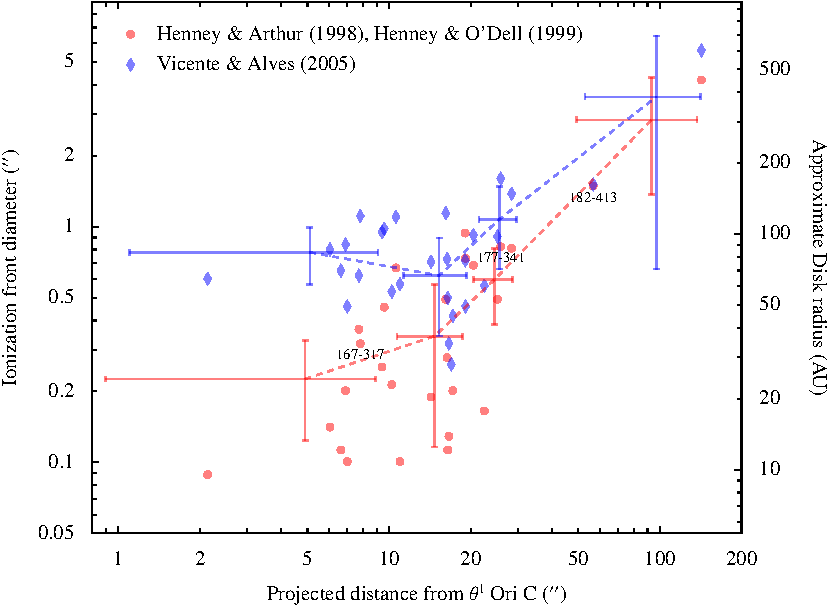
\includegraphics[width=\linewidth]{prop-size-2012}
  \caption{Variation with projected distance from the ionizing star of circumstellar disc sizes in the Orion proplyds.   Blue symbols show empirical determinations from \citet{Vicente:2005}, red symbols show results from fitting photoevaporation models \citep{Henney:1998, 1999AJ....118.2350H}.   The three proplyds that have been subject to gas-phase abundance studies are marked: 167-317 (LV~2), 177-341 (HST~1), a 182-413 (HST~10).   In only a few cases, such as HST~10, is the molecular disc size directly measured, for the rest it is assumed to be half the size of the ionization front.   Note that the \citeauthor{Vicente:2005} methodology significantly overestimates the true size of the ionization front (and by extension the enclosed disc) for proplyds that are much brighter than surrounding nebula, which tend to be those found close to the ionizing star.   Error bars show the mean and standard deviation measured in 4 broad spatial bins.}
  \label{fig:sizes}
\end{figure}
\begin{table*}\centering
  \caption{Comparison of physical properties between HST~10 and two other well-studied proplyds}
\label{tab:3props}
\setlength\tabcolsep{2\tabcolsep}
\begin{tabular}{llr rrr}\hline
 & Units & Note & LV~2 & HST~1 & HST~10 \\ \hline
Coordinate-based designation & & 1 & 167-317 & 177-341 & 182-413 \\
\rule{0pt}{3ex}\textit{Relation to ionizing source}\\
Projected distance, \(D'\) & \(''\) & 2 & 7.83 & 25.84 & 56.7 \\
Inclination, \(i\) & \(^\circ\) & 3 & 50 & 70 & 150 \\
True distance, \(D\) & pc & 4 & 0.022 & 0.059 & 0.242 \\
\rule{0pt}{3ex}\textit{Ionized cusp} \\
Ionization front radius, \(r_0\) & AU & 5 & 53. & 136. & 247. \\
Peak electron density, \(n_0\) & \(10^{6}\ \mathrm{cm^{-3}}\) & 6 & \(2.0\) & \(0.4\) & \(0.1\) \\
Ionization parameter &  & 7 & 0.012 & 0.008 & 0.002 \\
Cusp mass-loss rate, \(\dot{M}\) & \(10^{-7}\ M_\odot\ \mathrm{yr}^{-1}\) & 8 & \(2.6\) & \(2.5\) & \(2.1\) \\
\rule{0pt}{3ex}\textit{Molecular disc} \\
Disc effective temperature: \(T_\mathrm{d}\) & K & 9 & 95 & 58 & 29 \\
Disc mass \(M_\mathrm{d}\) & \(10^{-3}\ M_\odot\) & 10 & \(1.6\) & \(2.7\) & \(5.4\) \\
Disc radius \(R_\mathrm{d}\) & AU & 11 & 34 & 89 & 160 \\
% Sigma0(10 AU) & g/cm^2 & 7.57 & 5.06 & 5.59 \\
Evaporation time, \(t_\mathrm{evap}\) & \(10^4\ \mathrm{yr}\) & 12 & \(0.6\) & \(1.1\) & \(2.6\) \\
\hline
\end{tabular}
\par\smallskip
\begin{minipage}{0.7\linewidth}
  % \def\NoteSep{\\}
  \def\NoteSep{\quad}
  \textit{Notes}:\NoteSep 
  (1)~\citet{1994ApJ...436..194O}\NoteSep
  (2)~Angular separation from \thC{} \citep{1998AJ....115..263O}\NoteSep
  (3)~Inclination of proplyd axis to line of sight estimated from kinematic studies of the velocity--ionization correlation in emission lines from the cusp \citep{1999AJ....118.2350H, 2002ApJ...566..315H}.  Proplyds with \(i > 90^\circ\) have their head pointing away from the observer.\NoteSep
  (4)~\(D = D' / \sin i\).\NoteSep
  (5)~Estimated from fitting evaporation models to the \ha{} profiles of the cusps \cite{Henney:1998}.\NoteSep
  (6)~LV~2 from [\ion{C}{3}] density \citep{2002ApJ...566..315H}; HST~1 and HST~10 from model fitting (this paper and \citealp{Mesa-Delgado:2012}).\NoteSep
  (7)~\(F / (n_0\,c)\).\NoteSep 
  (8)~Calculated by integrating model mass fluxes over the area of the cusp.\NoteSep
  (9)~Radiative equilibrium temperature, assuming that 25\% of the bolometric flux from \thC{} reaches the surface of the disk (see also \citealp{Robberto:2002}).\NoteSep
  (10)~Estimated from observed fluxes at \(880~\mu\mathrm{m}\) \citep{Mann:2010} after subtracting the contribution from ionized free-free emission, assuming optically thin dust emission with opacity \(\kappa_\nu = 0.034~\mathrm{cm^2\ g^{-1}}\) and dust temperature equal to the effective temperatures derived above.\NoteSep
  (11)~Directly estimated from \textit{HST} images from HST~10.  For LV~2 and HST~1, we assume \(r_\mathrm{d} = 0.65 r_0\), see Figure~\ref{fig:sizes}.\NoteSep
  (12)~Nominal mass loss timescale: \(M_\mathrm{d} /\dot{M}\). 
\end{minipage}


\end{table*}

HST~10 is the third proplyd to be subject to a detailed abundance analysis, following earlier studies of LV~2 \citep{Tsamis:2011, Tsamis:2011a} and HST~1 \citep{Mesa-Delgado:2012}.  
These proplyds cover a broad range in size and in separation from the Trapezium stars (see Figure~\ref{fig:sizes}), and derived physical parameters for the three proplyds are summarised in Table~\ref{tab:model:pars}.  HST~10 shows a significantly lower ionization parameter than the two closer-in proplyds, which is reflected in its emission line spectrum that is relatively stronger in low ionization lines.  Despite these differences, the estimated mass loss rate from the ionized cusp is very similar for all three proplyds, being of order \(2 \times 10^{-7}\ M_\odot\ \mathrm{yr^{-1}}\).  These values are somewhat lower than earlier estimates (e.g., \citealp{1999AJ....118.2350H, 2002ApJ...566..315H}), which is partly because we are neglecting the contribution of mass loss though the proplyd tail.

Table~\ref{tab:3props} also shows estimates for the mass and radius of the embedded circumstellar accretion disk, which is the reservoir of mass in the proplyds.   All three proplyds show very similar sub-mm fluxes \citep{Mann:2010}, of order 20~mJy once the contribution from ionized free-free emission has been subtracted.  However, conversion of this flux to a gas mass requires knowledge of the dust opacity per unit gas mass  and dust temperature, both of which have large uncertainties \citep{Williams:2011b}.  The values in the table are calculated on the assumption that the dust temperature is the effective temperature of a disk in radiative equilibrium with the bolometric flux from the Trapezium stars,\footnote{Although the sub-mm emission is optically thin, the disks are likely to be optically thick at mid-infrared wavelengths where they emit the bulk of their radiation.   We assume that 50\% of the bolometric radiation from the Trapezium stars is absorbed in the ionized cusp of the proplyd, and that 50\% of the remainder is absorbed in the neutral photoevaporation flow, so that only 25\% reaches the surface of the disk.} and using the opacity recommended by \citep{Beckwith:1990} of \(0.1 (\nu/1000~\mathrm{GHz})~\mathrm{cm^2~g^{-1}}\), giving \(0.034~\mathrm{cm^2~g^{-1}}\) at 880~\(\mu\)m.   It must be emphasised that the derived masses are highly uncertain, since the opacity could be up to 20 times smaller if substantial grain growth up to cm-sized bodies has occured \citep{DAlessio:2001}.   Evidence for grain evolution has been found in the case of silhouette disks projected onto the Orion Nebula \citep{Miotello:2012}.   The masses given in the table are at least 6 times smaller than the ``minimum mass solar nebula'' \citep{Weidenschilling:1977a}, which is the mass within \(30\)~AU required to account for the composition of the planets in the Solar System.  

The nominal photoevaporation timescales, \(t_\mathrm{evap} = M_\mathrm{d}/\dot{M}\), are uncomfortably short compared with the estimated age of the photoionized nebula (\(\ge 10^5\)~yr; see discussion in \S~8.2.2 of \citealp{1999AJ....118.2350H}), but would come into agreement if the masses were increased by a factor of 5--10, which cannot be ruled out (see previous paragraph).   Interestingly, the evaporation timescale \(t_\mathrm{evap}\) \emph{increases} with increasing distance from the Trapezium.  Given that \(t_\mathrm{evap}\) should be roughly equal to the elapsed time since the disk photoevaporation commenced \citep{Johnstone:1998}, this is the opposite of what would be expected from a naive model of a roughly spherical \hii{} region, in which case proplyds at greater distances from the ionizing star would have entered the \hii{} region more recently.   However, evidence from both observations \citep{ODell:2009a} and numerical simulations \citep{Arthur:2011} point to the continued survival of dense clumps of molecular gas well inside the apparent boundary of the \hii{} region, in which case it is reasonable that the proplyds closest to the Trapezium might have been shielded from ultraviolet radiation until relatively recently.

The abundance results for the three proplyds are rather disparate, so that it is very hard to see any consistent trend in the results.   For instance, although we find a roughly solar oxygen abundance for HST~10 from both empirical analysis and photoevaporation model fitting, the oxygen abundance was found to be \(\simeq 3 \times\) super-solar in LV~2 \citep{Tsamis:2011} from a purely empirical analysis, with no discrepancy between collisional and recombination lines.  In contrast, \citet{Mesa-Delgado:2012} found oxygen to be \(\simeq 3 \times\) \emph{sub}-solar in HST~1, both from empirical analysis of CELs and from photoevaporation model fitting, whereas an empirical analysis of ORLs is more consistent with a solar value.   Given the wide range of characteristic ionization and density found in the three proplyds (Table~\ref{tab:3props}), it is possible that systematic errors in our abundance analysis might be contributing to this wide spread.   In order to rule out any such effects, it is vital to carry out a similar analysis on a sample of proplyds that all have \emph{similar} ionization parameters and densities.




\bibliographystyle{mn2e}
\bibliography{BibdeskLibrary}


\end{document}
